\documentclass[12pt,a4paper]{article}
\usepackage[margin=1in]{geometry}
\usepackage{graphicx}
\usepackage{booktabs}
\usepackage{longtable}
\usepackage{array}
\usepackage{float}
\usepackage{enumitem}
\usepackage{hyperref}
\usepackage{xcolor}
\usepackage{caption}
\usepackage{titlesec}
\usepackage{setspace}
\usepackage{microtype}
\hypersetup{colorlinks=true,linkcolor=black,urlcolor=blue,citecolor=black}
\setlength{\parskip}{0.45em}
\setlength{\parindent}{0pt}
\onehalfspacing
\titleformat{\section}{\large\bfseries}{\Roman{section}.}{0.5em}{}
\titleformat{\subsection}{\normalsize\bfseries}{\thesection.\Alph{subsection}.}{0.5em}{}
\renewcommand{\arraystretch}{1.22}
\newcommand{\projecttitle}{Comparative Analysis of Deep Learning Architectures for Sentiment Classification of Movie Reviews}

\begin{document}

\begin{titlepage}
\centering

\includegraphics[width=0.92\textwidth]{assets/logos/mitlogo.jpg}\par\vspace{1.6cm}
{\Large \textbf{FINAL REPORT}}\par\vspace{0.7cm}
{\LARGE \bfseries \projecttitle\par}\vspace{0.8cm}
{\large Deep Learning Project --- ICT-4442\par}\vspace{0.55cm}
{\small \textbf{GitHub Repository:} \url{https://github.com/sltrtn/imdb-sentiment-dl-comparison}\par}\vspace{0.8cm}
{\large \textbf{Submitted by}}\par\vspace{0.35cm}
\begin{tabular}{@{}l@{\hspace{2.4cm}}r@{}}
\textbf{Name} & \textbf{Registration No.}\\[0.15cm]
Hasil Haroon & 230953019\\
T Rama Mohan Aniketh & 230911224\\
Madhavan K & 230953298\\
Ayrton Pulikottil & 230953448\\
\end{tabular}
\vfill
{\large \textbf{School of Computer Engineering}}\par
{\large Manipal Institute of Technology, Manipal}\par
{\large Manipal Academy of Higher Education}\par\vspace{0.5cm}
{\large October 2026}
\end{titlepage}

\pagenumbering{roman}
\section*{Abstract}
Online-review sentiment classification helps organisations summarize customer feedback at a scale that manual reading cannot support. This project compares four architectures for binary sentiment classification of movie reviews: a TF--IDF multi-layer perceptron (MLP), a GloVe-initialised TextCNN, a GloVe-initialised bidirectional LSTM (BiLSTM), and a fine-tuned DistilBERT transformer. All models use the IMDB Large Movie Review Dataset and one common, leakage-free protocol: 22,500 training reviews, 2,500 validation reviews, and the untouched official 25,000-review test set. Hyperparameters are selected by validation F1 and the selected configuration is evaluated once on the test set. DistilBERT is the best model, achieving 0.9141 accuracy, 0.9138 F1, and 0.9723 ROC--AUC. The MLP remains a strong lightweight baseline at 0.8774 accuracy; TextCNN and BiLSTM reach 0.8718 and 0.8668 respectively. GloVe improves TextCNN accuracy from 0.8408 with random embeddings to 0.8718. Error analysis of DistilBERT shows reduced accuracy for the longest review quartile (0.8647) and for reviews containing negation cues (0.9081). The findings demonstrate the practical accuracy--compute trade-off between pretrained transformers and lighter models.

\noindent\textbf{Keywords---} sentiment analysis, IMDB, TextCNN, BiLSTM, DistilBERT, TF--IDF, GloVe, deep learning

\tableofcontents
\newpage
\pagenumbering{arabic}

\section{Introduction}
Online reviews are a major source of customer feedback, but manual review of thousands of documents is costly and inconsistent. Sentiment classification automates the task of assigning an overall positive or negative label to each review. The task is challenging because reviews can be long, informal, mixed in polarity, and sensitive to word order: ``not bad'' and ``not good'' have similar tokens but opposite meanings.

This mini project follows the scope stated in the synopsis and interim report. It compares four increasingly capable architectures on the same IMDB movie-review split: a TF--IDF MLP baseline, TextCNN, BiLSTM, and a fine-tuned DistilBERT. The interim report documented the common data pipeline and preliminary MLP/TextCNN results; the final work completes the planned GloVe integration, BiLSTM, DistilBERT, hyperparameter selection, common evaluation, and error analysis.

\section{Literature Review}
Maas et al. introduced the balanced IMDB dataset and showed the enduring value of bag-of-words features for review sentiment \cite{maas}. Wang and Manning showed that strong lexical baselines remain competitive \cite{wang}. Distributed representations such as word2vec \cite{mikolov} and GloVe \cite{glove} provide semantically useful embedding initialisation for neural classifiers.

Kim's TextCNN applies multiple convolution widths and max pooling to text classification \cite{kim}. LSTM cells were designed to preserve information across long sequences \cite{lstm}; document-sentiment work subsequently demonstrated the value of gated recurrent encoders \cite{tang}. Attention-based Transformers \cite{vaswani} enabled pretrained language models such as BERT \cite{bert}, while DistilBERT reduces the cost of BERT through knowledge distillation \cite{distilbert}. The data-cleaning, optimization, and regularisation choices in this study are also informed by Adam \cite{adam}, dropout \cite{dropout}, and the original TF--IDF formulation \cite{salton}.

The literature motivates a controlled comparison instead of assuming that a larger model is automatically preferable. Classical representations can be highly effective, while pretrained transformers may better resolve context and long-range dependencies at a higher compute cost.

\section{Objectives}
\begin{enumerate}[label=\arabic*.]
\item Implement and compare MLP, TextCNN, BiLSTM, and fine-tuned DistilBERT under one common IMDB evaluation protocol.
\item Measure test accuracy, precision, recall, F1, ROC--AUC, parameter count, and selected-run training time to quantify the performance--cost trade-off.
\item Analyse the strongest model's failures by review length and negation cues, and identify practical limitations of the comparison.
\end{enumerate}

\section{Methodology}
\subsection{Shared data pipeline}
The IMDB Large Movie Review Dataset contains 50,000 labelled English reviews, balanced between positive and negative classes \cite{maas}. The original official training and test partitions contain 25,000 reviews each. Since the Stanford download endpoint was inaccessible in the experiment environment, the implementation reads the official \texttt{stanfordnlp/imdb} Hugging Face mirror and caches its parquet files locally; it also supports a local \texttt{aclImdb} release.

HTML tags are removed, line breaks are replaced, repeated whitespace is collapsed, and no review is discarded. The official training partition is shuffled once with seed 42 and split into 22,500 training and 2,500 validation reviews. The official test partition remains untouched until final evaluation. All vocabulary fitting and model selection use training/validation data only.

\subsection{MLP + TF--IDF}
The baseline represents each review with up to 20,000 TF--IDF unigram and bigram features, with \texttt{min\_df=2} and English stop words removed. A one-hidden-layer ReLU \texttt{MLPClassifier} is trained with Adam, batch size 128, early stopping, and a maximum of 30 iterations. Hidden-layer size (128 or 256) and L2 regularisation are selected on validation F1. This establishes a strong non-sequential reference model.

\subsection{TextCNN}
Following Kim \cite{kim}, TextCNN lowercases and tokenizes each review, maps tokens to 100-dimensional embeddings, and applies parallel one-dimensional convolutions with widths 3, 4, and 5. Global max pooling, dropout (0.5), and a linear binary classifier produce the final prediction. The search compares random embeddings at 200 tokens with fine-tuned 100-dimensional GloVe embeddings at 200 and 300 tokens. The best configuration uses GloVe, 300 tokens, and 128 filters per kernel width.

\subsection{BiLSTM}
The BiLSTM uses a 50,000-token training vocabulary and 100-dimensional GloVe embeddings. Sequences are truncated to 256 tokens, dynamically padded in batches, and packed by true length so that padding does not affect recurrence. The model concatenates the final forward and backward hidden states, applies dropout, and classifies with a linear head. Three configurations vary hidden width, dropout, learning rate, and whether GloVe is frozen; gradients are clipped to norm 5.

\subsection{DistilBERT}
The transformer model is \texttt{distilbert-base-uncased}, fine-tuned end to end with its two-class classification head \cite{distilbert}. The pretrained WordPiece tokenizer truncates/pads each review to 256 tokens. Training uses AdamW with weight decay 0.01, a linear schedule with 10\% warm-up, batch size 32, gradient clipping at norm 1, bfloat16 autocast on GPU, and three epochs. Learning rates $2\times10^{-5}$ and $3\times10^{-5}$ are compared on validation F1.

\section{Experimental Setup}
\textbf{Hardware and software.} Experiments ran on a 12th Gen Intel Core i5-12450H, 15 GB RAM, and NVIDIA GeForce RTX 3050 Laptop GPU (6 GB). The implementation uses Python 3.14, PyTorch 2.14.1, Transformers 5.22, scikit-learn 1.9, and CUDA 13.0.

\textbf{Metrics and selection.} Accuracy, positive-class precision, recall, F1, ROC--AUC, and the $2\times2$ confusion matrix are reported. Within each family, the configuration with highest validation F1 is selected. The test set is used only once for the selected configuration. Seeds for Python, NumPy, PyTorch, and the split are fixed at 42.

\section{Results and Discussion}
\begin{table}[H]
\centering\small
\caption{Final performance on the official 25,000-review IMDB test set.}
\begin{tabular}{lrrrrrrr}
\toprule
Model & Acc. & Prec. & Recall & F1 & AUC & Params & Time (s)\\
\midrule
DistilBERT & \textbf{0.9141} & \textbf{0.9174} & 0.9102 & \textbf{0.9138} & \textbf{0.9723} & 66,955,010 & 643\\
MLP + TF--IDF & 0.8774 & 0.8780 & 0.8766 & 0.8773 & 0.9477 & 2,560,257 & 73\\
TextCNN + GloVe & 0.8718 & 0.8523 & \textbf{0.8995} & 0.8753 & 0.9439 & 2,154,369 & 24\\
BiLSTM + GloVe & 0.8668 & 0.8509 & 0.8895 & 0.8698 & 0.9387 & 5,117,777 & 40\\
\bottomrule
\end{tabular}
\end{table}

\begin{figure}[H]
\centering
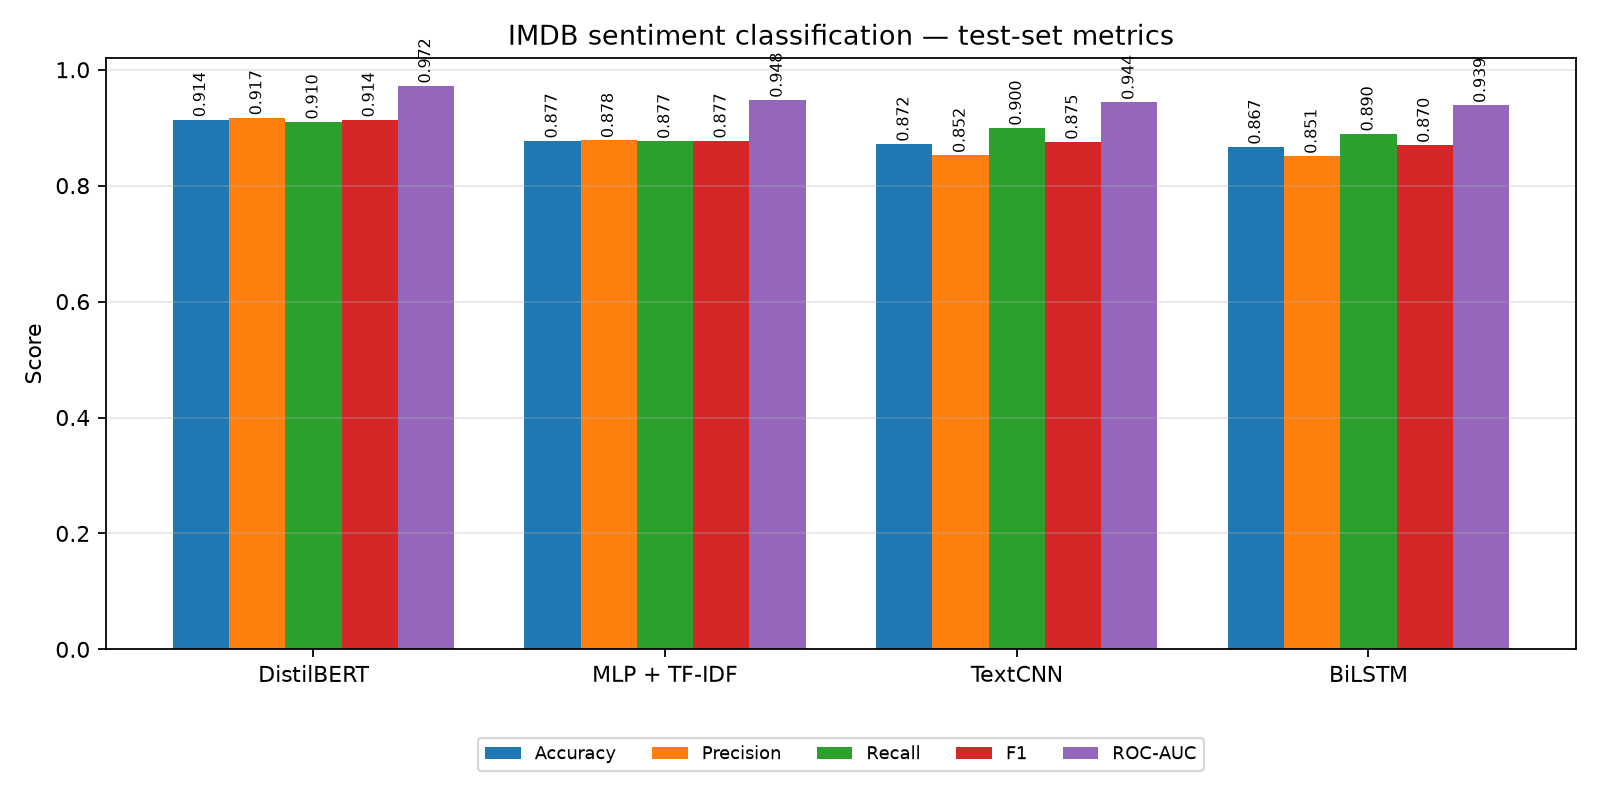
\includegraphics[width=\textwidth]{results/figures/metric_comparison.png}
\caption{Test-set metric comparison.}
\end{figure}

DistilBERT has the best result on every aggregate metric and improves accuracy by 3.7 percentage points over the strongest non-transformer, the MLP. Its pretrained contextual representation is particularly helpful when sentiment depends on composition rather than isolated phrases. The cost is substantial: the selected run has 67.0M parameters and takes 643 seconds, versus 2.56M parameters and 73 seconds for the MLP. The timing is hardware-specific, but illustrates the trade-off that motivated the project.

The MLP's 0.8774 accuracy confirms that sparse lexical features are a serious baseline for IMDB. TextCNN and BiLSTM both have higher recall than precision, indicating a mild tendency to predict positive reviews. TextCNN offers the best accuracy-per-second among the neural sequence models. GloVe is clearly useful: random-initialized TextCNN reaches 0.8408 accuracy, while the selected GloVe configuration reaches 0.8718.

\begin{figure}[H]
\centering
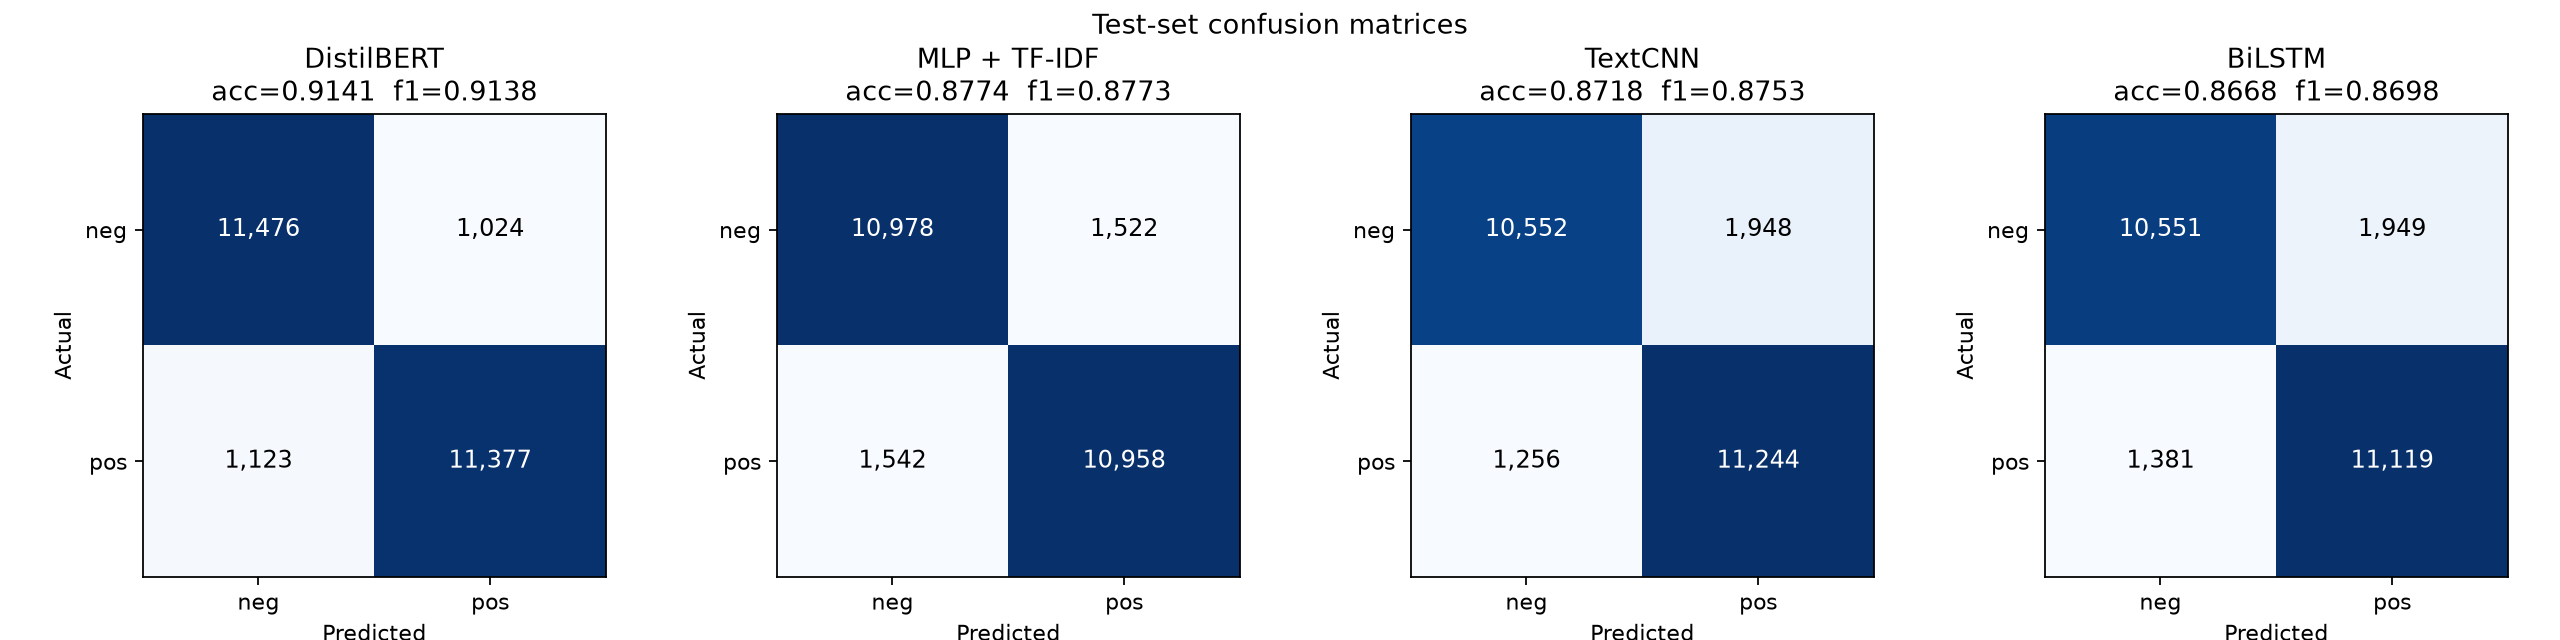
\includegraphics[width=0.95\textwidth]{results/figures/confusion_matrices.png}
\caption{Confusion matrices for the selected models.}
\end{figure}

\subsection{Hyperparameter selection}
\begin{table}[H]
\centering\footnotesize
\caption{Validation-selected configurations and held-out test results.}
\begin{tabular}{llrrr}
\toprule
Family & Selected configuration & Val. F1 & Test acc. & Test F1\\
\midrule
MLP & 128 hidden units, $\alpha=10^{-3}$ & 0.8917 & 0.8774 & 0.8773\\
TextCNN & GloVe, 300 tokens, 128 filters & 0.8913 & 0.8718 & 0.8753\\
BiLSTM & 128 hidden units, fine-tuned GloVe & 0.8824 & 0.8668 & 0.8698\\
DistilBERT & $2\times10^{-5}$ learning rate & 0.9148 & 0.9141 & 0.9138\\
\bottomrule
\end{tabular}
\end{table}

\subsection{Error analysis}
The selected DistilBERT checkpoint correctly classifies 22,853 of 25,000 test reviews. Accuracy is stable for the first three length quartiles but falls substantially for reviews of 274--2,235 words. This is consistent with the model's 256-token limit and the more mixed sentiment often present in long reviews. Negation cues are also associated with a higher error rate.

\begin{table}[H]
\centering
\caption{DistilBERT error slices on the test set.}
\begin{tabular}{lrr}
\toprule
Slice & Reviews & Accuracy\\
\midrule
4--124 words & 6,214 & 0.9340\\
125--169 words & 6,192 & 0.9381\\
170--273 words & 6,320 & 0.9201\\
274--2,235 words & 6,274 & 0.8647\\
Contains negation cue & 18,743 & 0.9081\\
No negation cue & 6,257 & 0.9322\\
\bottomrule
\end{tabular}
\end{table}

\begin{figure}[H]
\centering
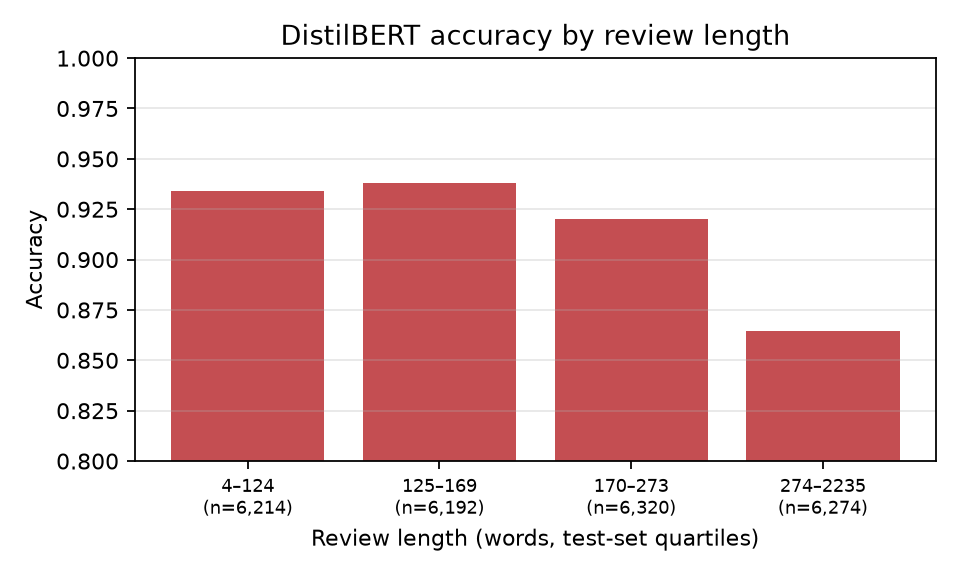
\includegraphics[width=0.72\textwidth]{results/figures/accuracy_by_length.png}
\caption{DistilBERT accuracy by test-review length quartile.}
\end{figure}

Some of the most confident apparent mistakes contain strong sentiment language that contradicts their assigned label, which is consistent with noisy labels or deliberately ironic/mixed reviews. This limits what an aggregate metric can reveal and motivates retaining qualitative error analysis.

\section{Conclusion}
The project completed the four-model comparison proposed in the synopsis and interim report under a shared, reproducible IMDB protocol. Fine-tuned DistilBERT is the most accurate model, achieving 0.9141 test accuracy and 0.9138 F1. The MLP, TextCNN, and BiLSTM remain strong lower-cost alternatives, with the GloVe TextCNN offering the best neural-model speed/accuracy balance. Pretraining, rather than architectural complexity alone, accounts for much of DistilBERT's advantage.

\section{Future Work}
Future experiments should repeat each configuration across multiple seeds and report confidence intervals. Chunking or hierarchical encoding could reduce the long-review truncation issue. Larger hyperparameter searches, layer-wise learning rates, and additional pretrained encoders could improve transformer performance. Finally, cross-domain evaluation on product, social-media, or multilingual reviews would test robustness beyond the saturated IMDB benchmark.

\section*{Acknowledgement}
We thank the School of Computer Engineering, Manipal Institute of Technology, for the guidance and computational resources that supported this project.

\begin{thebibliography}{99}
\bibitem{maas} A. L. Maas et al., ``Learning Word Vectors for Sentiment Analysis,'' in \emph{Proceedings of ACL}, 2011, pp. 142--150.
\bibitem{wang} S. Wang and C. D. Manning, ``Baselines and Bigrams: Simple, Good Sentiment and Topic Classification,'' in \emph{Proceedings of ACL}, 2012, pp. 90--94.
\bibitem{mikolov} T. Mikolov et al., ``Efficient Estimation of Word Representations in Vector Space,'' arXiv:1301.3781, 2013.
\bibitem{glove} J. Pennington, R. Socher, and C. D. Manning, ``GloVe: Global Vectors for Word Representation,'' in \emph{Proceedings of EMNLP}, 2014, pp. 1532--1543.
\bibitem{kim} Y. Kim, ``Convolutional Neural Networks for Sentence Classification,'' in \emph{Proceedings of EMNLP}, 2014, pp. 1746--1751.
\bibitem{lstm} S. Hochreiter and J. Schmidhuber, ``Long Short-Term Memory,'' \emph{Neural Computation}, vol. 9, no. 8, pp. 1735--1780, 1997.
\bibitem{tang} D. Tang, B. Qin, and T. Liu, ``Document Modeling with Gated Recurrent Neural Network for Sentiment Classification,'' in \emph{Proceedings of EMNLP}, 2015, pp. 1422--1432.
\bibitem{vaswani} A. Vaswani et al., ``Attention Is All You Need,'' in \emph{Advances in Neural Information Processing Systems}, 2017.
\bibitem{bert} J. Devlin et al., ``BERT: Pre-training of Deep Bidirectional Transformers for Language Understanding,'' in \emph{Proceedings of NAACL-HLT}, 2019, pp. 4171--4186.
\bibitem{distilbert} V. Sanh et al., ``DistilBERT, a Distilled Version of BERT: Smaller, Faster, Cheaper and Lighter,'' arXiv:1910.01108, 2019.
\bibitem{adam} D. P. Kingma and J. Ba, ``Adam: A Method for Stochastic Optimization,'' in \emph{Proceedings of ICLR}, 2015.
\bibitem{dropout} N. Srivastava et al., ``Dropout: A Simple Way to Prevent Neural Networks from Overfitting,'' \emph{JMLR}, vol. 15, no. 1, pp. 1929--1958, 2014.
\bibitem{salton} G. Salton and C. Buckley, ``Term-weighting Approaches in Automatic Text Retrieval,'' \emph{Information Processing \& Management}, vol. 24, no. 5, pp. 513--523, 1988.
\end{thebibliography}

\clearpage
\section*{Individual Contribution Statement}
\addcontentsline{toc}{section}{Individual Contribution Statement}
\begin{longtable}{p{0.22\textwidth}p{0.16\textwidth}p{0.45\textwidth}p{0.12\textwidth}}
\toprule
Member & Registration No. & Contribution & Signature\\
\midrule
\endfirsthead
\toprule
Member & Registration No. & Contribution & Signature\\
\midrule
\endhead
Hasil Haroon & 230953019 & Shared data pipeline; TF--IDF vectorisation; MLP baseline; experiment tracking. & \\
T Rama Mohan Aniketh & 230911224 & TextCNN implementation; GloVe embedding integration; convolutional-model tuning. & \\
Madhavan K & 230953298 & BiLSTM implementation; packing/padding strategy; recurrent-model tuning. & \\
Ayrton Pulikottil & 230953448 & DistilBERT fine-tuning; tokenizer integration; common evaluation and error analysis. & \\
\bottomrule
\end{longtable}

\end{document}
